% !TeX TXS-program:compile = txs:///arara
% arara: lualatex: {shell: yes, synctex: yes, interaction: batchmode}
% arara: pythontex: {rerun: modified} if found('pytxcode', 'PYTHONTEX#py')
% arara: lualatex: {shell: yes, synctex: yes, interaction: batchmode} if found('pytxcode', 'PYTHONTEX#py')
% arara: lualatex: {shell: yes, synctex: yes, interaction: batchmode} if found('log', '(undefined references|Please rerun|Rerun to get)')

\documentclass[a4paper,11pt]{article}
\usepackage[]{cp-base}
\graphicspath{{./graphics/}}
%variables
\donnees[%
	typedoc=CHAPITRE~,
	numdoc=11,
	classe=1\up{ère} 2M2,
	matiere={[SPÉ.MATHS]},
	annee=2022,
	titre={Applications de la dérivation}
	]

%formatage
\author{Pierquet}
\title{\nomfichier}
\hypersetup{pdfauthor={Pierquet},pdftitle={\nomfichier},allbordercolors=white,pdfborder=0 0 0,pdfstartview=FitH}
%divers
\lhead{\entete{\matiere}}
\chead{\entete{\lycee}}
\rhead{\entete{\classe{} - Chapitre \thepart}}
\lfoot{\pied{\matiere}}
\cfoot{\logolycee{}}
\rfoot{\pied{\numeropagetot}}
\fancypagestyle{entetedm}{\fancyhead[L]{\entete{\matiere{} À rendre avant le ...}}}
\fancypagestyle{enteteds}{\fancyhead[L]{\entete{Durée : \duree}}}

\tikzset{tangent/.style={% https://tex.stackexchange.com/a/25940
		decoration={%
			markings,mark=at position #1 with{
				\coordinate (tangent point-\pgfkeysvalueof{/pgf/decoration/mark info/sequence number}) at (0pt,0pt);
				\coordinate (tangent unit vector-\pgfkeysvalueof{/pgf/decoration/mark info/sequence number}) at (1,0pt);
				\coordinate (tangent orthogonal unit vector-\pgfkeysvalueof{/pgf/decoration/mark info/sequence number}) at (0pt,1);}
		},
		postaction=decorate},
	use tangent/.style={shift=(tangent point-#1),%
		x=(tangent unit vector-#1),
		y=(tangent orthogonal unit vector-#1)
	},
	use tangent/.default=1}

\begin{document}

\pagestyle{fancy}

\part{CH11 - Applications de la dérivation}

\section{Lien entre dérivée et tangente}

\subsection{Rappels}

\begin{crappel}[s]
Le \textbf{nombre dérivé} $f'(a)$ d'une fonction $f$ en $a$ est le coefficient directeur de la tangente à la courbe représentative de $f$ au point d’abscisse $a$.

\smallskip

Une fonction affine est croissante si et seulement si son coefficient directeur est positif.

\smallskip

La tangente en $A$ à une courbe est la droite qui s'approche le mieux de la courbe au voisinage de A.
\end{crappel}

\subsection{Théorème fondamental}

\begin{cthm}
Soit $f$ une fonction définie et dérivable sur un intervalle $I$. Alors :
\begin{itemize}
	\item la fonction $f$ est croissante sur $I$ $\ssi$ sa dérivée $f'$ est positive sur $I$ ;
	\item la fonction $f$ est décroissante sur $I$ $\ssi$ sa dérivée $f'$ est négative sur $I$ ;
	\item la fonction $f$ est constante sur $I$ $\ssi$ sa dérivée $f'$ est nulle sur $I$ tout entier.
\end{itemize}
\end{cthm}

\begin{crmq}
Ce théorème s’énonce aussi au sens strict (strictement croissante avec strictement positive, \ldots)
\end{crmq}

\begin{cdemo}
On a vu que le nombre dérivé en $a$ est le coefficient directeur de la tangente au voisinage du point d'abscisse $a$. Comme cette tangente est la droite qui s'approche le mieux de la courbe, la courbe et la tangente on le même sens de variation au voisinage de $a$. Et comme le signe du coefficient directeur d'une droite donne les variations de celle-ci, le signe de $f'(a)$ donne le sens de variation de $f$ au voisinage de $a$.
\end{cdemo}

\begin{cillustr}
\begin{center}
	\begin{tikzpicture}[x=1cm,y=0.5cm]
		%styles
		\tkzSetUpPoint[shape=circle,size=4pt,color=violet,fill=violet]
		\tikzset{tan style/.style={<->,>=latex}}
		\tkzInit[xmin=-2,xmax=8,xstep=1,ymin=-4,ymax=6.1,ystep=1]
		%courbe
		\tkzFct[very thick,red,domain=-2:8,samples=250]{2*cos(2*x)+cos(x)+3*cos(3*x)};
		%tangentes croissantes
		\foreach \x/\lg in {-1/0.25,2/0.3,4/0.75,6/0.15}{\tkzDrawTangentLine[very thick,color=blue,kr=\lg,kl=\lg](\x)}
		%tangentes décroissantes
		\foreach \x/\lg in {1/0.25,3/0.3,5/0.3}{\tkzDrawTangentLine[very thick,color=ForestGreen,kr=\lg,kl=\lg](\x)}
		%tangente hor
		\tkzDrawTangentLine[very thick,color=darkgray,kr=0.75,kl=0.75](0)
		%points
		\foreach \va in {-1,0,1,2,3,4,5,6}{\tkzDefPointByFct[draw](\va)}
	\end{tikzpicture}
\end{center}
On peut donc constater que :
\begin{itemize}
	\item les \og {\blue tangentes bleues montent} \fg{} et que la courbe \og suit la même direction \fg{} ;
	\item les \og \textcolor{ForestGreen}{tangentes vertes descendent} \fg{} et que la courbe \og suit la même direction \fg{} ;
	\item la \og \textcolor{darkgray}{tangente grise est horizontale} \fg{} et que la courbe \og change de direction \fg{}.
\end{itemize}
La tangente et la courbe vont donc dans la \og même direction \fg{} !
\end{cillustr}

\subsection{Une méthode très importante}

\begin{cmethode}
Pour étudier les variations d'une fonction :
\begin{itemize}
	\item on \textbf{calcule sa fonction dérivée} $f'$ en utilisant la formule adéquate ;
	\item on \textbf{étudie le signe de cette dérivée} (en général en faisant un \textbf{tableau de signes}) ;
	\item on \textbf{conclut} grâce au théorème ci-dessus ; 
	\item on calcule les extremums de la fonction (ce qui est au \og bout des flèches \fg), en calculant les images des nombres qui sont dans la première ligne, quand on peut.
\end{itemize}
\end{cmethode}

\begin{crmq}[s]
Cette méthode fait donc appels à plusieurs chapitres et notions étudiées précédemment :
\begin{itemize}
	\item dérivation globale pour calculer la dérivée d'une fonction ;
	\item équations, inéquations, et tableaux de signes pour le signe de la dérivée ;
	\item calculatrice pour les images et la courbe.
\end{itemize}
\end{crmq}

\begin{cexemple}
Déterminer les variations de la fonction $f$ définie sur $\R$ par $f(x)=2x^3+3x^2-12x+5$.
\begin{itemize}
	\item La fonction $f$ est sous la forme d'une somme, donc on la dérive terme à terme :
	
	$f'(x)=2 \times 3x^2 + 3 \times 2x -12=6x^2+6x-12$.
	\item La dérivée est un polynôme du second degré, donc on sait étudier son signe ; on calcule $ \Delta$, les racines, et on regarde le signe de $a=6$ :
	\begin{center}
		\begin{tikzpicture}
			\tkzTabInit[lgt=4]{$x$/1,$f'(x)=6x^2+6x-12$/1}{$-\infty$,$-2$,$1$,$+\infty$}
			\tkzTabLine{,+,z,-,z,+,}
		\end{tikzpicture}
	\end{center}
	\item On en déduit que la fonction $f$ est croissante sur $\intervOF{-\infty}{-2}$ et sur $\intervFO{1}{+\infty}$ et décroissante sinon.
	\item Il reste à calculer les extremums de la fonction : $f(-2)=2 \times (-2)^3 + 3 \times (-2)^2 - 12 \times (-2)+5=25$ et $f(1)=-2$. 
	
	On obtient alors le tableau suivant :
	\begin{center}
		\begin{tikzpicture}
			\def\tkzTabDefaultBackgroundColor{SeaGreen!5}
			\tkzTabInit[lgt=4]{$x$ / 1 , $f'(x)=6x^2+6x-12$ / 1, $f$ /2}{$-\infty$, $-2$, $1$, $+\infty$}
			\tkzTabLine{,+ , z, - ,z ,+ ,}
			\tkzTabVar{-/ , +/ 25  ,  -/ $-2$  ,  +/}	
		\end{tikzpicture}	
	\end{center}		
\end{itemize}
\textit{Attention à ne pas se tromper d'expression quand on remplace : c'est une ligne qui concerne $f$ donc on remplace dans $f(x)$ et pas dans $f'$.}
\end{cexemple}

\begin{cexercice}
Dresser le tableau de variations de la fonction $f$ définie sur $\R$ par $f(x)=\dfrac{1}{x^2+1}$ en utilisant la méthode décrite précédemment.

Vérifier en traçant la courbe de cette fonction sur la calculatrice.
\end{cexercice}

\section{Optimisation}

\subsection{Définition}

\begin{cdefi}[s]
Une fonction $f$ admet un \textbf{minimum} sur un intervalle $I$ si l’une de ses images est plus petite que toutes les autres :

\hfill{}$f$ admet un minimum sur $I$ $\ssi$ il existe $x_0 \in I$ tel que $f (x)  \pg f (x_0)$ pour tout $x \in I$.\hfill{}

\smallskip

Il y a une définition équivalente pour un \textbf{maximum}.

\smallskip

On appelle \textbf{extremum} une valeur extrême, c’est-à-dire un minimum ou un maximum.
\end{cdefi}

\subsection{Propriété}

\begin{cprop}
Soit $f$ une fonction dérivable sur un intervalle $I$.

Si $f$ admet un extremum en $x_0$, alors $f'$ s'annule pour $x=x_0$.
\end{cprop}

\begin{cattention}
La réciproque est fausse : ce n'est pas parce que la dérivée s'annule que la fonction admet un extremum !

\smallskip

Par exemple voyons ce qui se passe avec la fonction cube $f(x)=x^3$ qui a pour dérivée $f'(x)=3x^2$.

\begin{minipage}{0.7\linewidth}
	\begin{center}
		\begin{tikzpicture}
			\def\tkzTabDefaultBackgroundColor{red!10}
			\tkzTabInit[lgt=3]{$x$/1,$f'(x)$/1,$f$/2}{$-\infty$,$0$,$+\infty$}
			\tkzTabLine{,+,z,+,}
			\tkzTabVar{-/,R/,+/}
			\tkzTabIma{1}{3}{2}{0}
		\end{tikzpicture} 
	\end{center}	
\end{minipage}\hfill%
\begin{minipage}{0.3\linewidth}
	\vspace{0.25cm}
	\begin{center}
		\tunits{1}{1}
		\tdefgrille{-2}{2}{1}{1}{-2}{2}{1}{1}
		\begin{tikzpicture}[x=\xunit cm,y=\yunit cm]
			\axestikz*[width=1pt] ;
			\axextikz[width=1pt,size=\scriptsize]{-2,-1,1} ; \axeytikz[width=1pt,size=\scriptsize]{-2,-1,1} ;
			\draw (-1pt,-1pt) node[below left] {\scriptsize $0$} ;
			\clip (\xmin,\ymin) rectangle (\xmax,\ymax) ;
			\draw[line width=1pt,samples=200,domain=\xmin:\xmax,red] plot (\x,{\x*\x*\x}) ;
		\end{tikzpicture}
	\end{center}
\end{minipage}
En $0$, la dérivée s'annule mais la fonction ne change pas de variation car la dérivée ne change pas de signe. Cela signifie que la courbe va présenter un \og plat \fg{} au niveau de 0 mais restera toujours strictement croissante !
\end{cattention}

\begin{cmethode}
Les problèmes dits d'\textbf{optimisation} sont les problèmes qui consistent à chercher le minimum ou le maximum d'une fonction. Ce sont des préoccupations quotidiennes ! (limiter les coûts, les besoins en matériaux, maximiser les bénéfices, les rendements, \ldots)

Dès qu'on cherche à optimiser (minimiser ou maximiser) une fonction, il faut en fait chercher les variations de cette fonction, avec la méthode donnée plus haut.
\end{cmethode}

\begin{chistoire}
\vspace{-0.22cm}
\lettrine[findent=.5em,nindent=0pt,lines=3,image,novskip=0pt]{newton}{}La construction de la notion de \textbf{dérivation} (et ses applications) n’a pas été un long fleuve tranquille. L’Europe de la fin du XXII\up{e} siècle a été le théâtre d’un affrontement scientifique entre deux écoles de pensée, d’un côté le monde anglais véhicule les « fluxions » de Newton tandis que le reste de l’Europe porte la pensée de Leibniz. 

Voici comment, dans son ouvrage (1687), Newton exprime sa vision des dérivées :

« Les rapports ultimes dans lesquels les quantités disparaissent ne sont pas réellement des rapports de quantités ultimes, mais les limites vers lesquelles les rapports de quantités, décroissant sans limite, s’approchent toujours, et vers lesquelles ils peuvent s’approcher aussi près qu’on veut. »

\smallskip

\hfill\textit{\tiny Tiré du BARBAZO de 1\up{ère}, 2019}
\end{chistoire}

\end{document}